\documentclass[journal]{IEEEtran}
\usepackage[T1]{fontenc}
\usepackage[utf8]{inputenc}
\usepackage{graphicx}
\usepackage{booktabs}
\usepackage{array}
\usepackage{url}
\usepackage[hidelinks]{hyperref}
\usepackage{stfloats}
\graphicspath{{figures/}}
\renewcommand{\thefigure}{S\arabic{figure}}
\renewcommand{\thetable}{S\Roman{table}}

\begin{document}
\title{Supplementary Material: Single-Channel EEG Detection of N3 Sleep with Interpretable Slow-Wave Factor Scores}
\markboth{Supplementary material}{Supplementary material}
\maketitle

\noindent This supplement follows the order of the Results in the main text; the tag at the start of each caption gives the research question it supports. All values come from run \texttt{20261030-1528}, and the complete tables are in the repository folder \texttt{v2/results/20261030-1528}. Analyses marked post hoc were added after the first complete run and do not enter any prespecified verdict.

\begin{center}\scriptsize
\begin{tabular}{@{}>{\raggedright\arraybackslash}p{2.7cm}>{\raggedright\arraybackslash}p{2.9cm}>{\raggedright\arraybackslash}p{2.0cm}@{}}
\toprule
Topic (main text) & Figures & Tables \\
\midrule
Baselines (III-D, IV-B) & -- & SI \\
Detection (IV-A, IV-B) & S1 curves, S2 calibration, S3 participants & -- \\
Factor scores (IV-C, IV-D) & S4 decline, S5 N2 vs N3 & SIII grade shares \\
Stability and profile (IV-F, IV-J) & S6 minutes and retest, S10 example night & SIV agreement (ICC) \\
Components (IV-G) & S7 leave-one-out & SII effects \\
Explanations (IV-H) & S8 band importance & -- \\
Reliability (IV-I) & S9 selective prediction & SV inputs \\
Robustness (IV-K) & -- & SVI sensitivity \\
\bottomrule
\end{tabular}
\end{center}

\begin{table}[!h]
\caption{\textbf{[Baselines (Section IV-B)]} Deviations of the re-implemented baselines from their published training recipes. All share the folds, inner selection, temperature scaling, threshold rule, loss, class weight and augmentation of the proposed model.}
\centering\scriptsize
\begin{tabular}{@{}p{1.8cm}p{6.3cm}@{}}
\toprule
Model & Implementation and deviations \\
\midrule
DeepSleepNet & Dual-branch CNN (small and large filters) with two BiLSTM(512) layers and residual shortcut; trained end-to-end on 64-epoch sequences instead of the two-step schedule. \\
TinySleepNet & CNN (128 filters, 4 layers) with LSTM(128); 64-epoch sequences instead of 15--20; common amplitude/noise augmentation instead of signal shifts. \\
AttnSleep & Multi-resolution CNN, feature recalibration and causal temporal context encoder for 100~Hz; epoch-wise as published; weighted binary instead of weighted categorical cross-entropy; encoder in 32-bit precision. \\
L-SeqSleepNet & STFT input, learnable filterbank, BiGRU epoch encoder and long-sequence encoder; 64 epochs folded into 8 subsequences of 8 instead of 200 as 20 of 10. \\
\bottomrule
\end{tabular}
\end{table}

\begin{figure*}[!t]
\centering
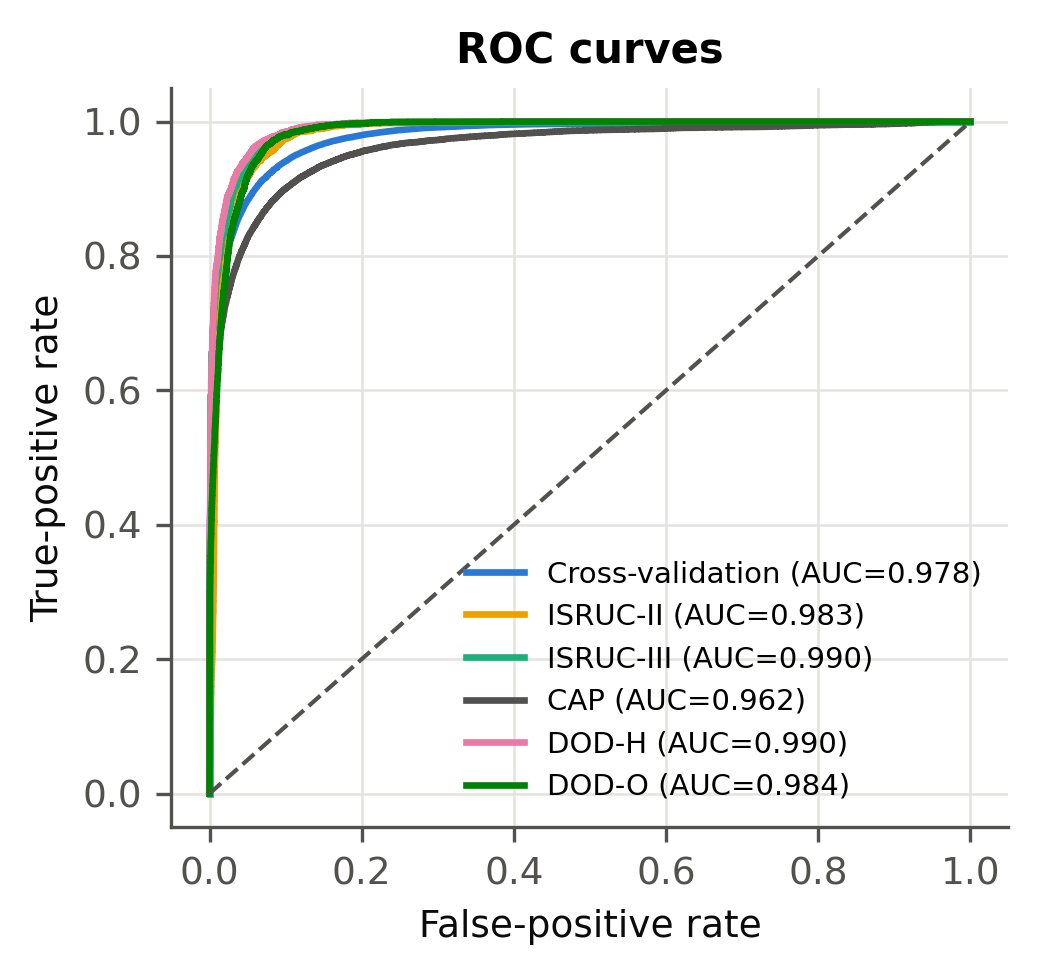
\includegraphics[width=0.44\textwidth]{fig_rq1_roc_curves.png}\hfill
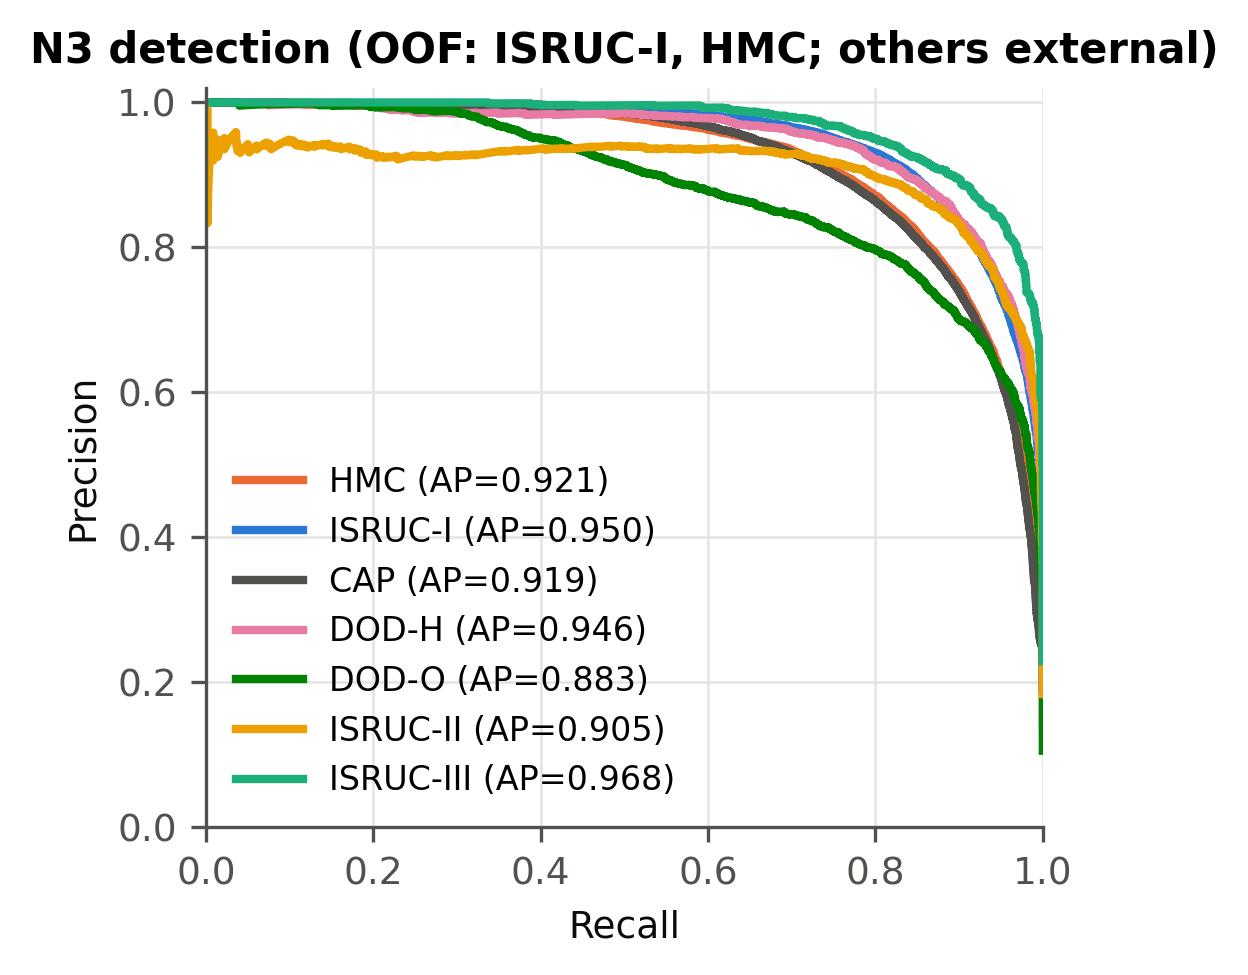
\includegraphics[width=0.44\textwidth]{fig_rq1_pr_curves.png}
\caption{ROC curves (left) and precision--recall curves (right) per cohort.}
\label{fig:s1}
\end{figure*}

\begin{figure*}[!t]
\centering
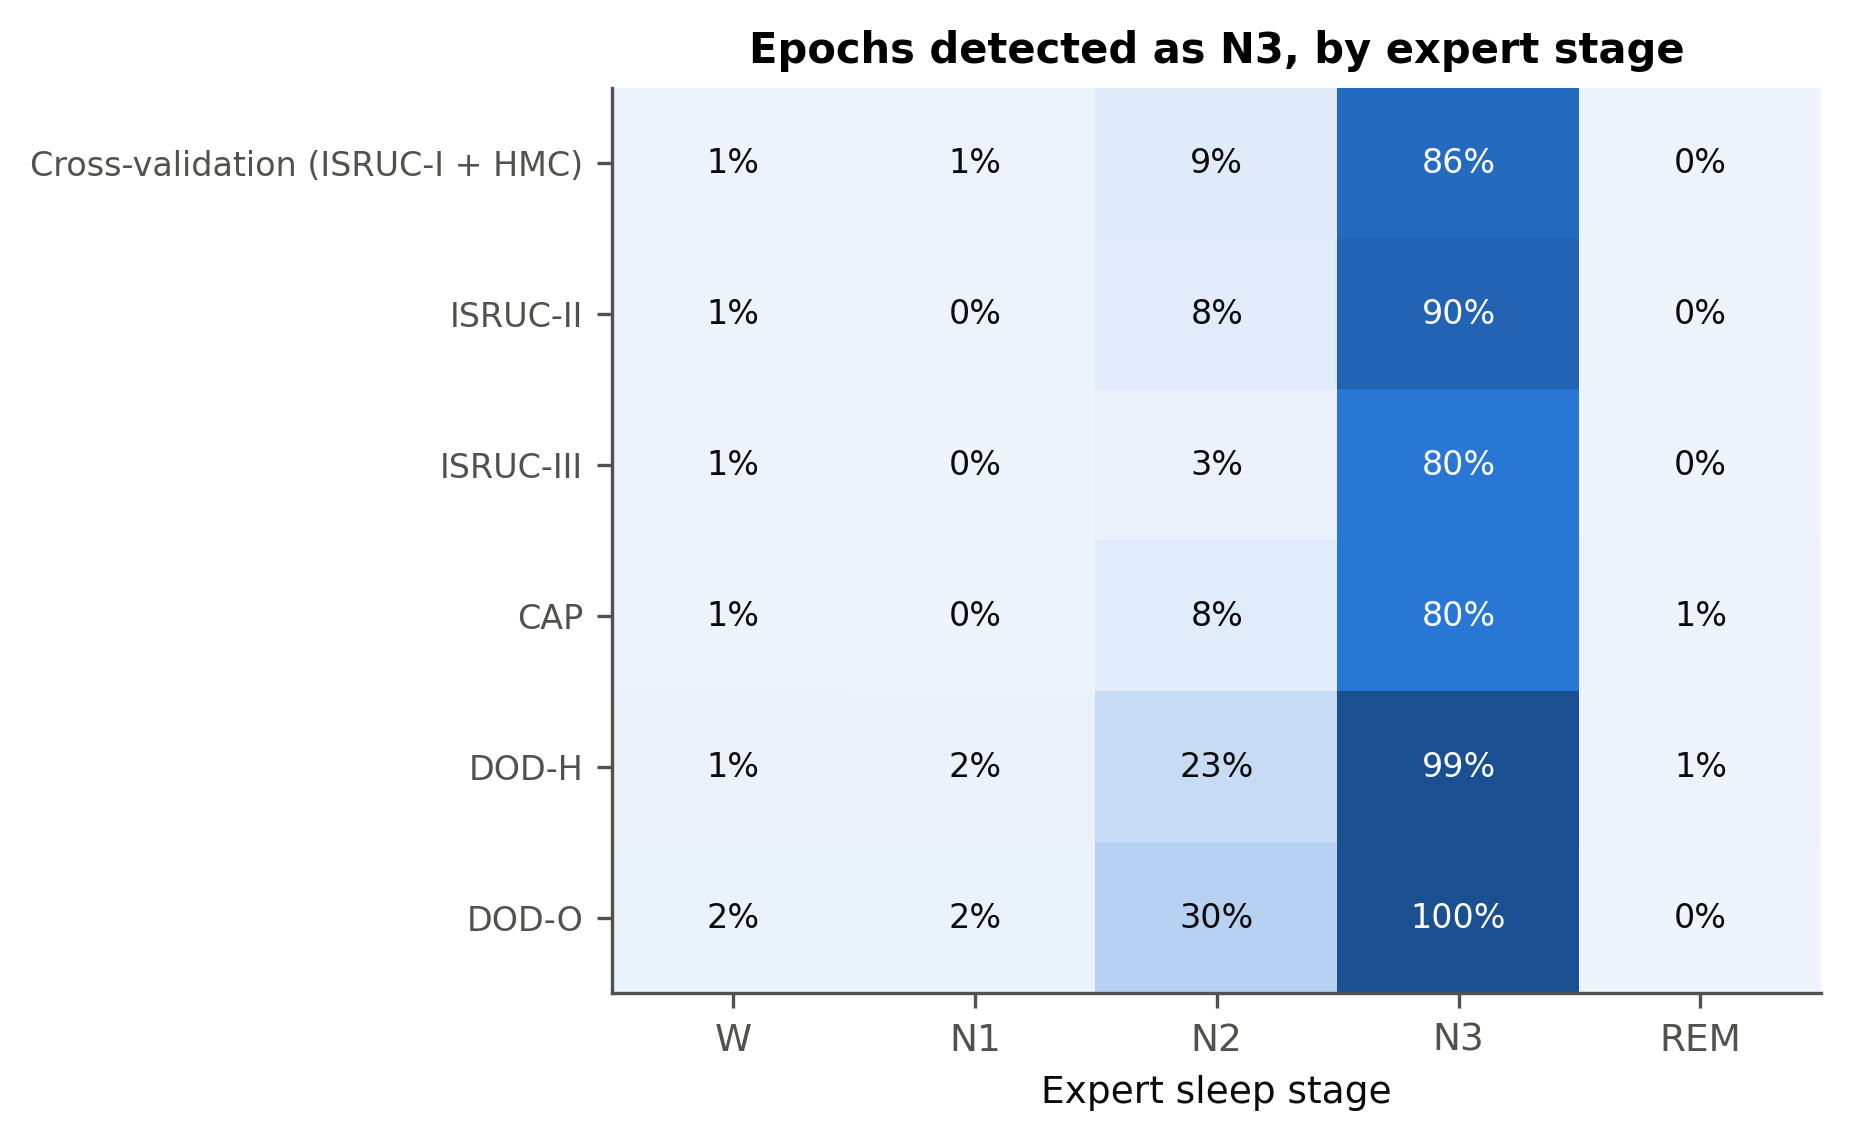
\includegraphics[width=0.44\textwidth]{fig_rq1_n3_by_expert_stage.png}\hfill
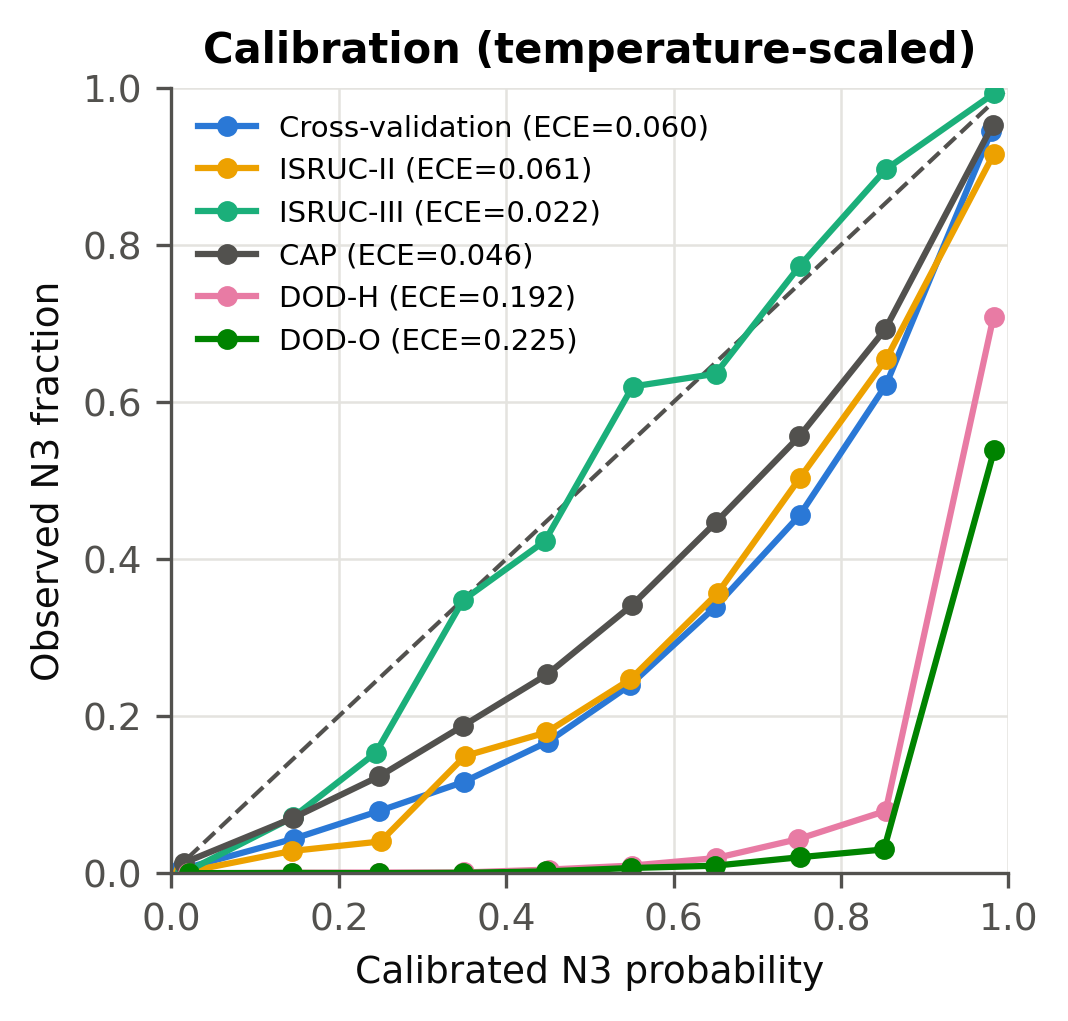
\includegraphics[width=0.44\textwidth]{fig_rq1_calibration.png}
\caption{Left: share of epochs of each expert stage predicted as N3. Right: reliability diagram of the temperature-scaled N3 probability with expected calibration error per cohort.}
\label{fig:s3}
\end{figure*}

\begin{figure*}[!t]
\centering
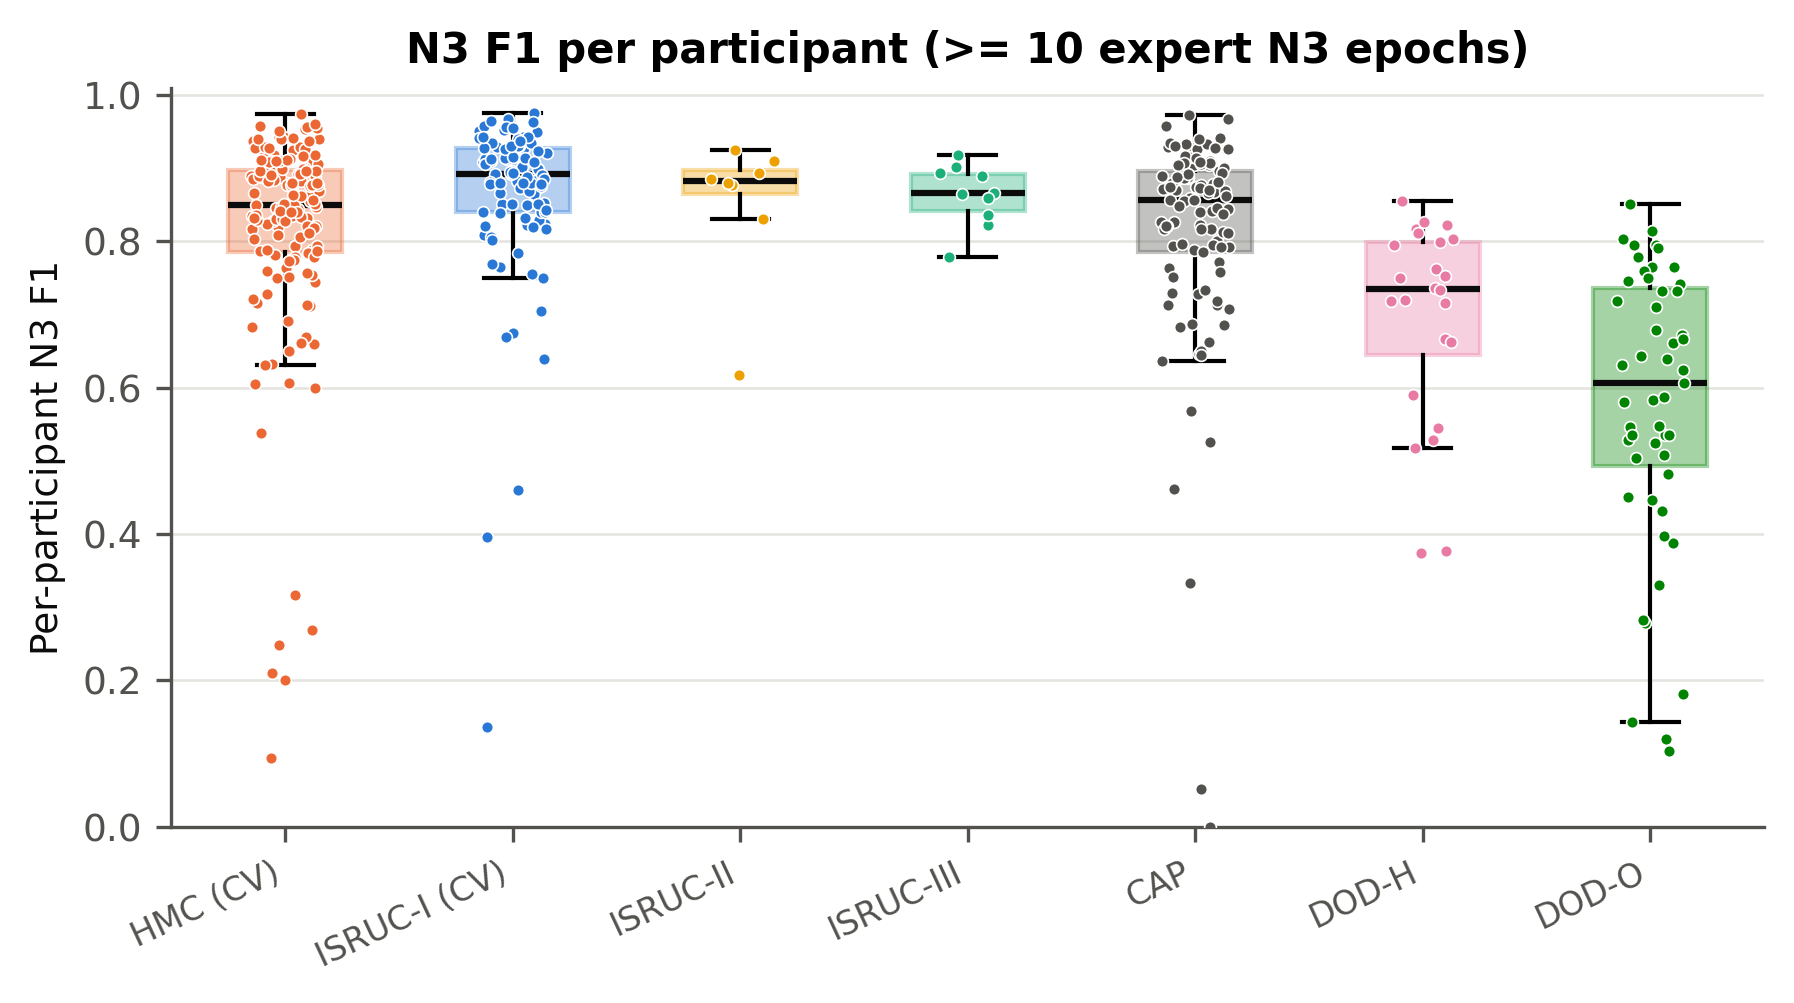
\includegraphics[width=0.44\textwidth]{fig_rq1_participant_f1.png}\hfill
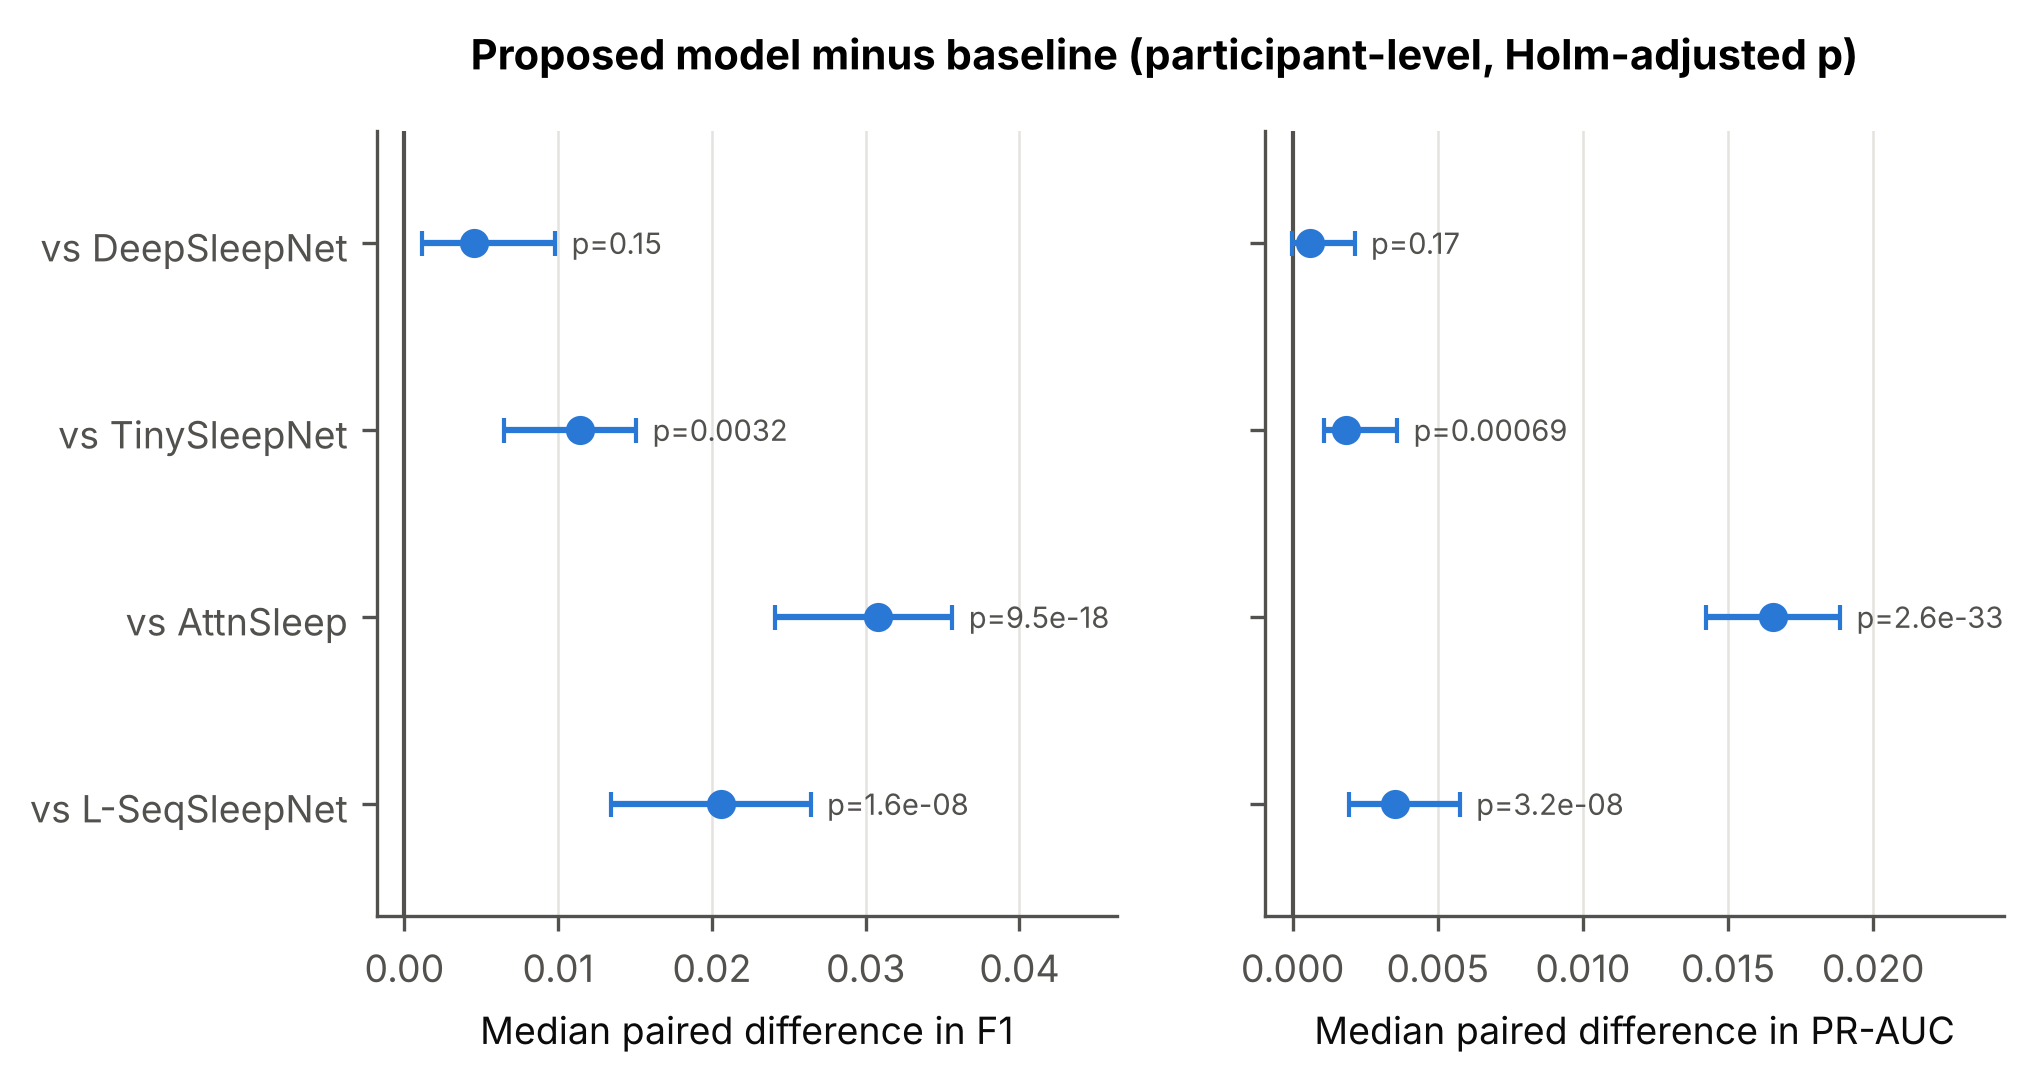
\includegraphics[width=0.44\textwidth]{fig_rq1_sota_forest.png}
\caption{Left: participant-level F1 scores (participants with at least 10 expert N3 epochs). Right: paired participant-level differences between the proposed model and each baseline with 95\% CI and Holm-corrected $p$.}
\end{figure*}

\begin{table}[!t]
\caption{Component effects: median paired participant difference in F1 (with minus without), 95\% CI and Holm-corrected $p$. Upper block prespecified; lower block post hoc, from the full model, with its own Holm family.}

\centering
\setlength{\tabcolsep}{3pt}
\scriptsize
\begin{tabular}{@{}lcc@{}}
\toprule
Component & $\Delta$F1 (95\% CI) & $p$ \\
\midrule
Feature fusion (no context) & +0.003 ($-$0.001, 0.006) & 1 \\ % rq4_component_effects.csv
Class weighting (no context) & 0.000 ($-$0.003, 0.003) & 1 \\
Attention vs mean pooling & $-$0.003 ($-$0.006, 0.000) & 0.34 \\
Temporal context & +0.023 (0.018, 0.027) & $<$0.001 \\
CNN vs features-only boosting & +0.036 (0.030, 0.043) & $<$0.001 \\
\midrule
Feature fusion (full model) & +0.007 (0.003, 0.011) & 0.018 \\ % rq4_extended_component_effects.csv
Class weighting (full model) & 0.000 ($-$0.003, 0.004) & 1 \\
Attention (full model) & +0.003 (0.000, 0.006) & 1 \\
Context $\pm$15 vs $\pm$3 epochs & +0.003 (0.001, 0.005) & 1 \\
All 19 vs 10 delta features & +0.002 ($-$0.002, 0.004) & 1 \\
\bottomrule
\end{tabular}
\end{table}

\begin{figure}[!t]
\centering
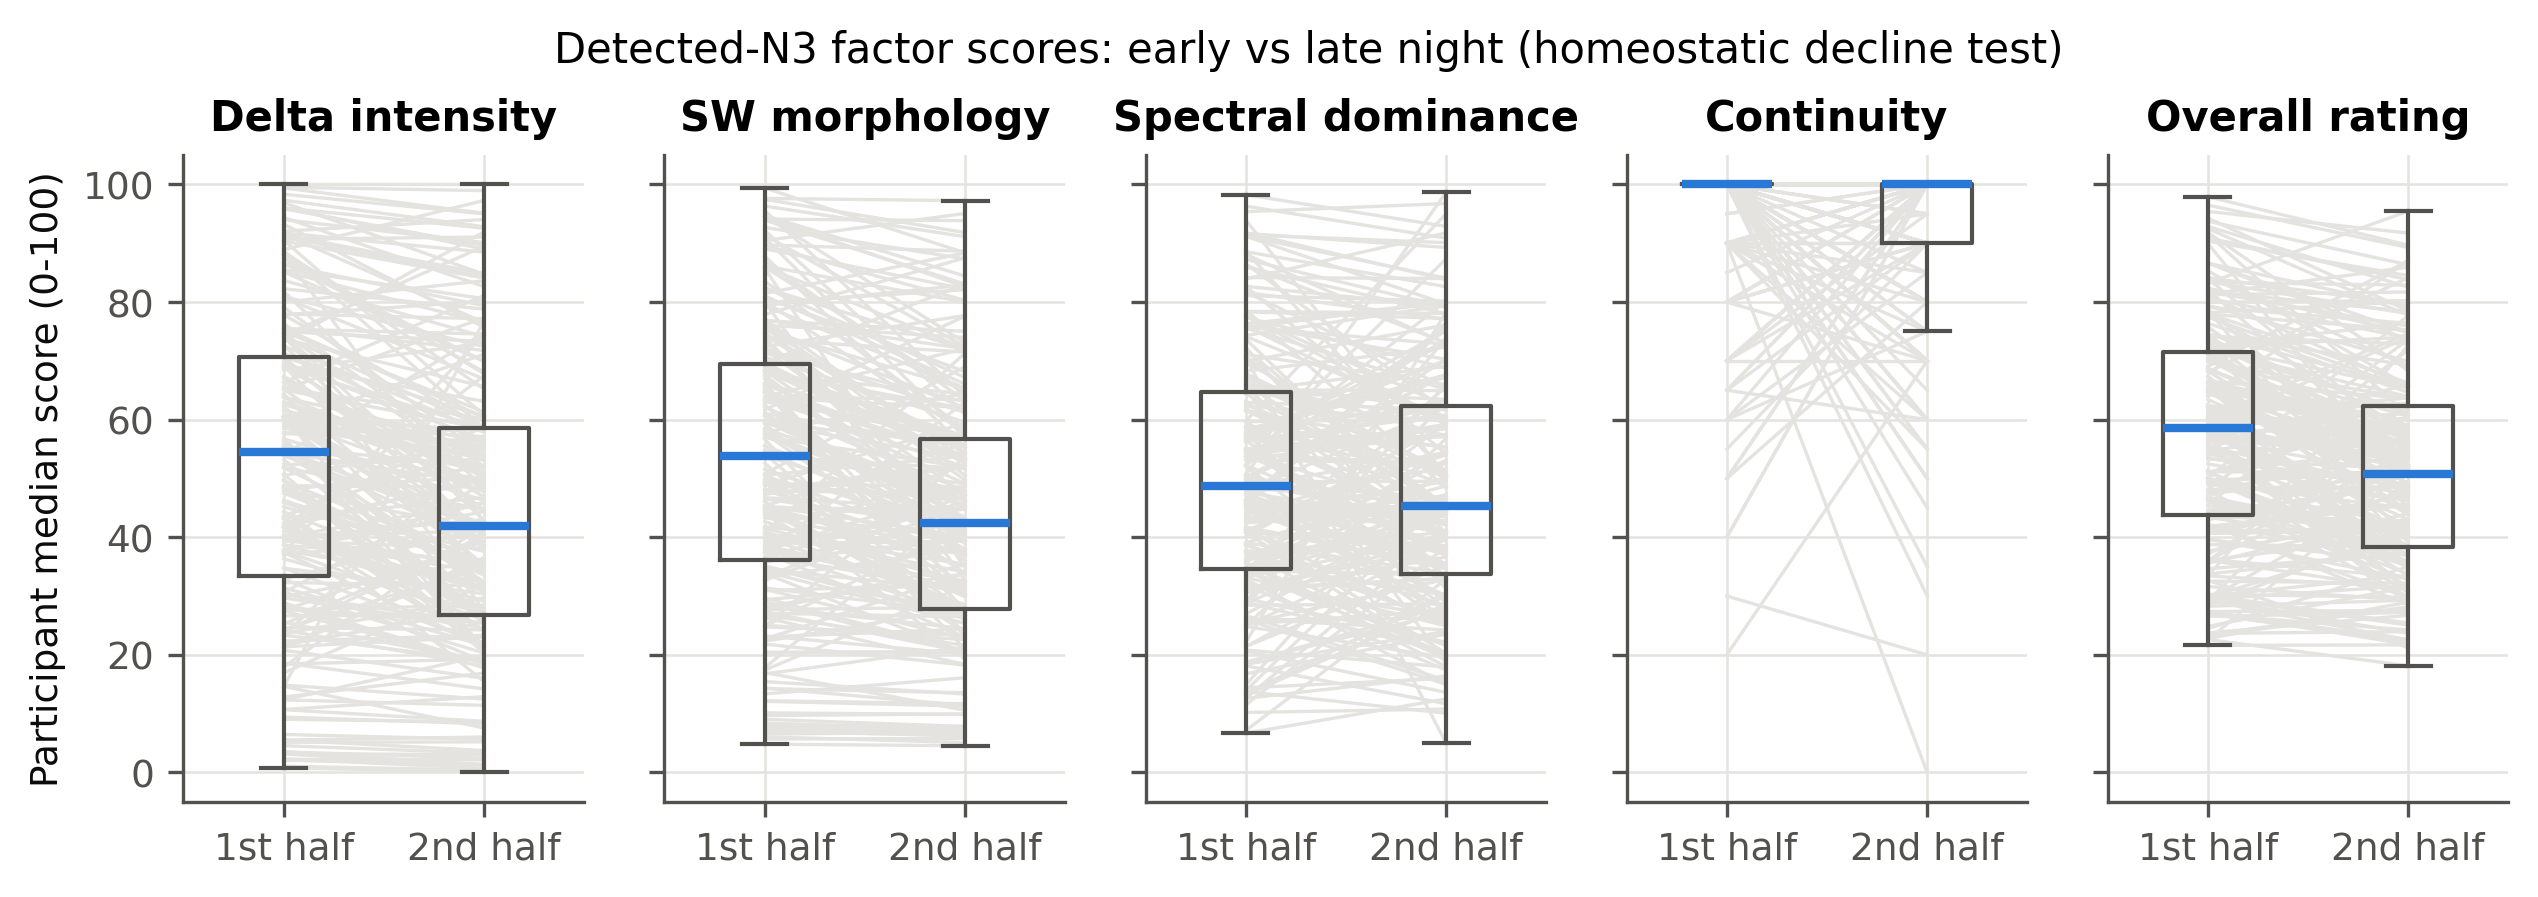
\includegraphics[width=0.86\columnwidth]{fig_rq2_early_vs_late.png}
\caption{Participant median factor scores of detected N3 in the first and second half of the night (cross-validation).}
\end{figure}

\begin{figure}[!t]
\centering
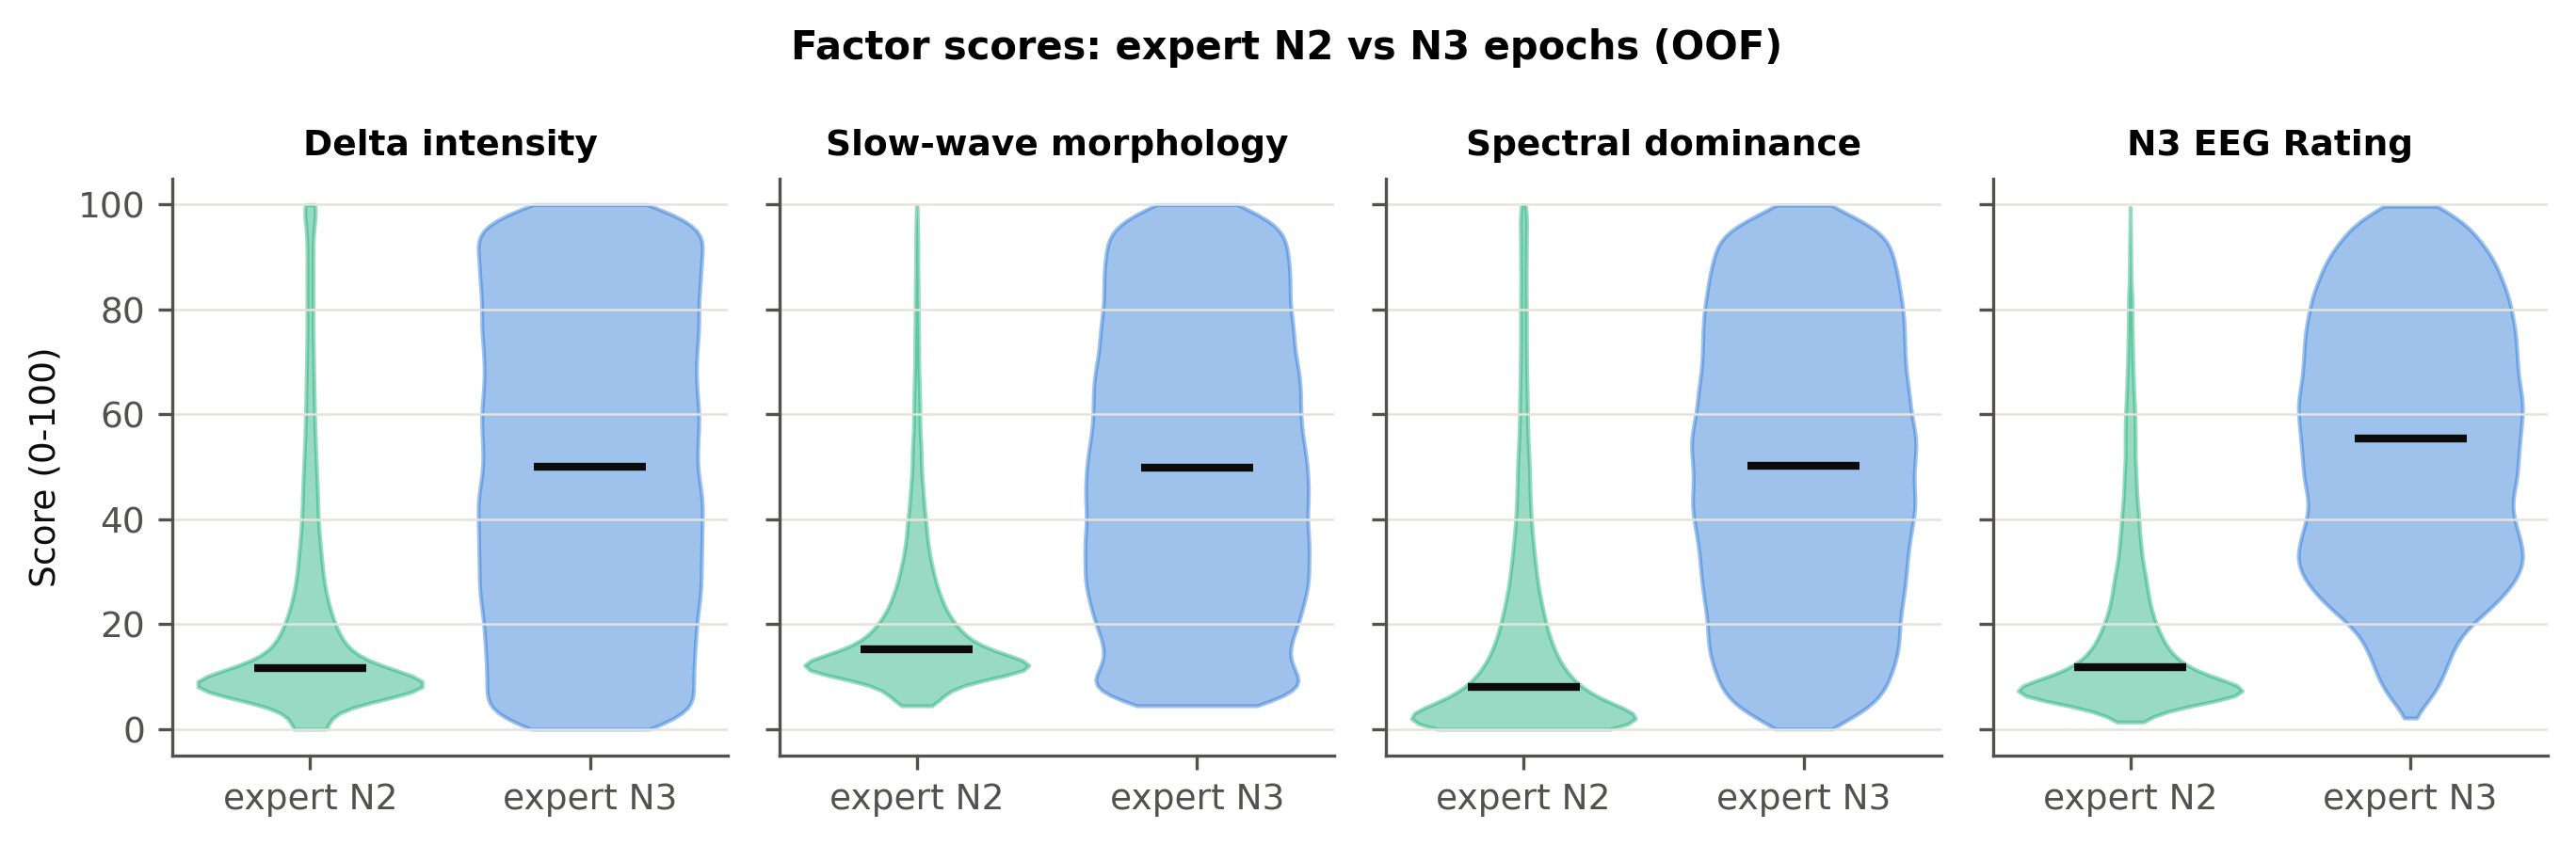
\includegraphics[width=0.86\columnwidth]{fig_rq2_factors_by_stage.png}
\caption{Factor scores of expert N2 and expert N3 epochs (cross-validation).}
\end{figure}

\begin{figure*}[!t]
\centering
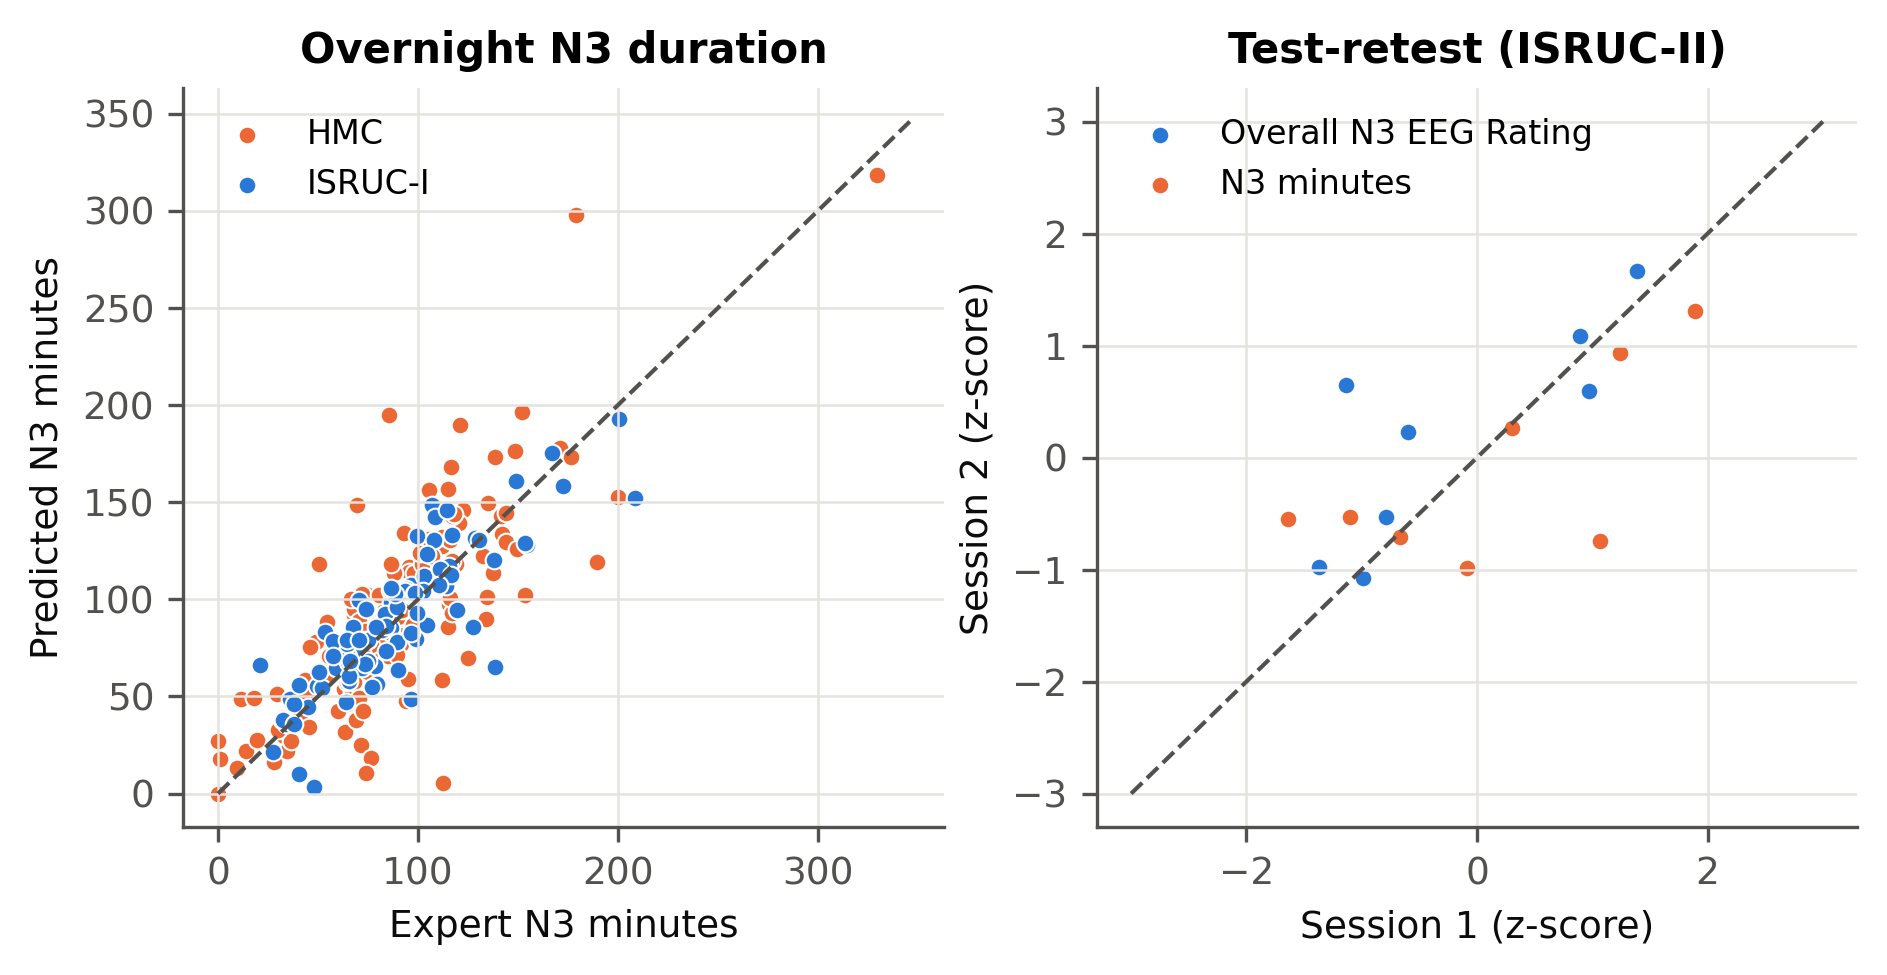
\includegraphics[width=0.56\textwidth]{fig_rq7_profiles.png}
\caption{Predicted vs expert N3 minutes per night (left) and ISRUC-II test--retest of the rating and of N3 minutes (right). Bland--Altman plots are in Fig.~4 of the main text.}
\end{figure*}

\begin{table}[!t]
\caption{Slow-wave grade distribution of detected N3 epochs (share of epochs).}
\centering\scriptsize
\begin{tabular}{@{}lccc@{}}
\toprule
Cohort & Low & Moderate & High \\
\midrule
HMC (CV) & 0.529 & 0.377 & 0.094 \\
ISRUC-I (CV) & 0.653 & 0.285 & 0.062 \\
CAP & 0.523 & 0.353 & 0.124 \\
DOD-H & 0.560 & 0.359 & 0.081 \\
DOD-O & 0.746 & 0.215 & 0.039 \\
ISRUC-II & 0.625 & 0.289 & 0.086 \\
ISRUC-III & 1.000 & 0.000 & 0.000 \\
\bottomrule
\end{tabular}
\end{table}

\begin{figure}[!t]
\centering
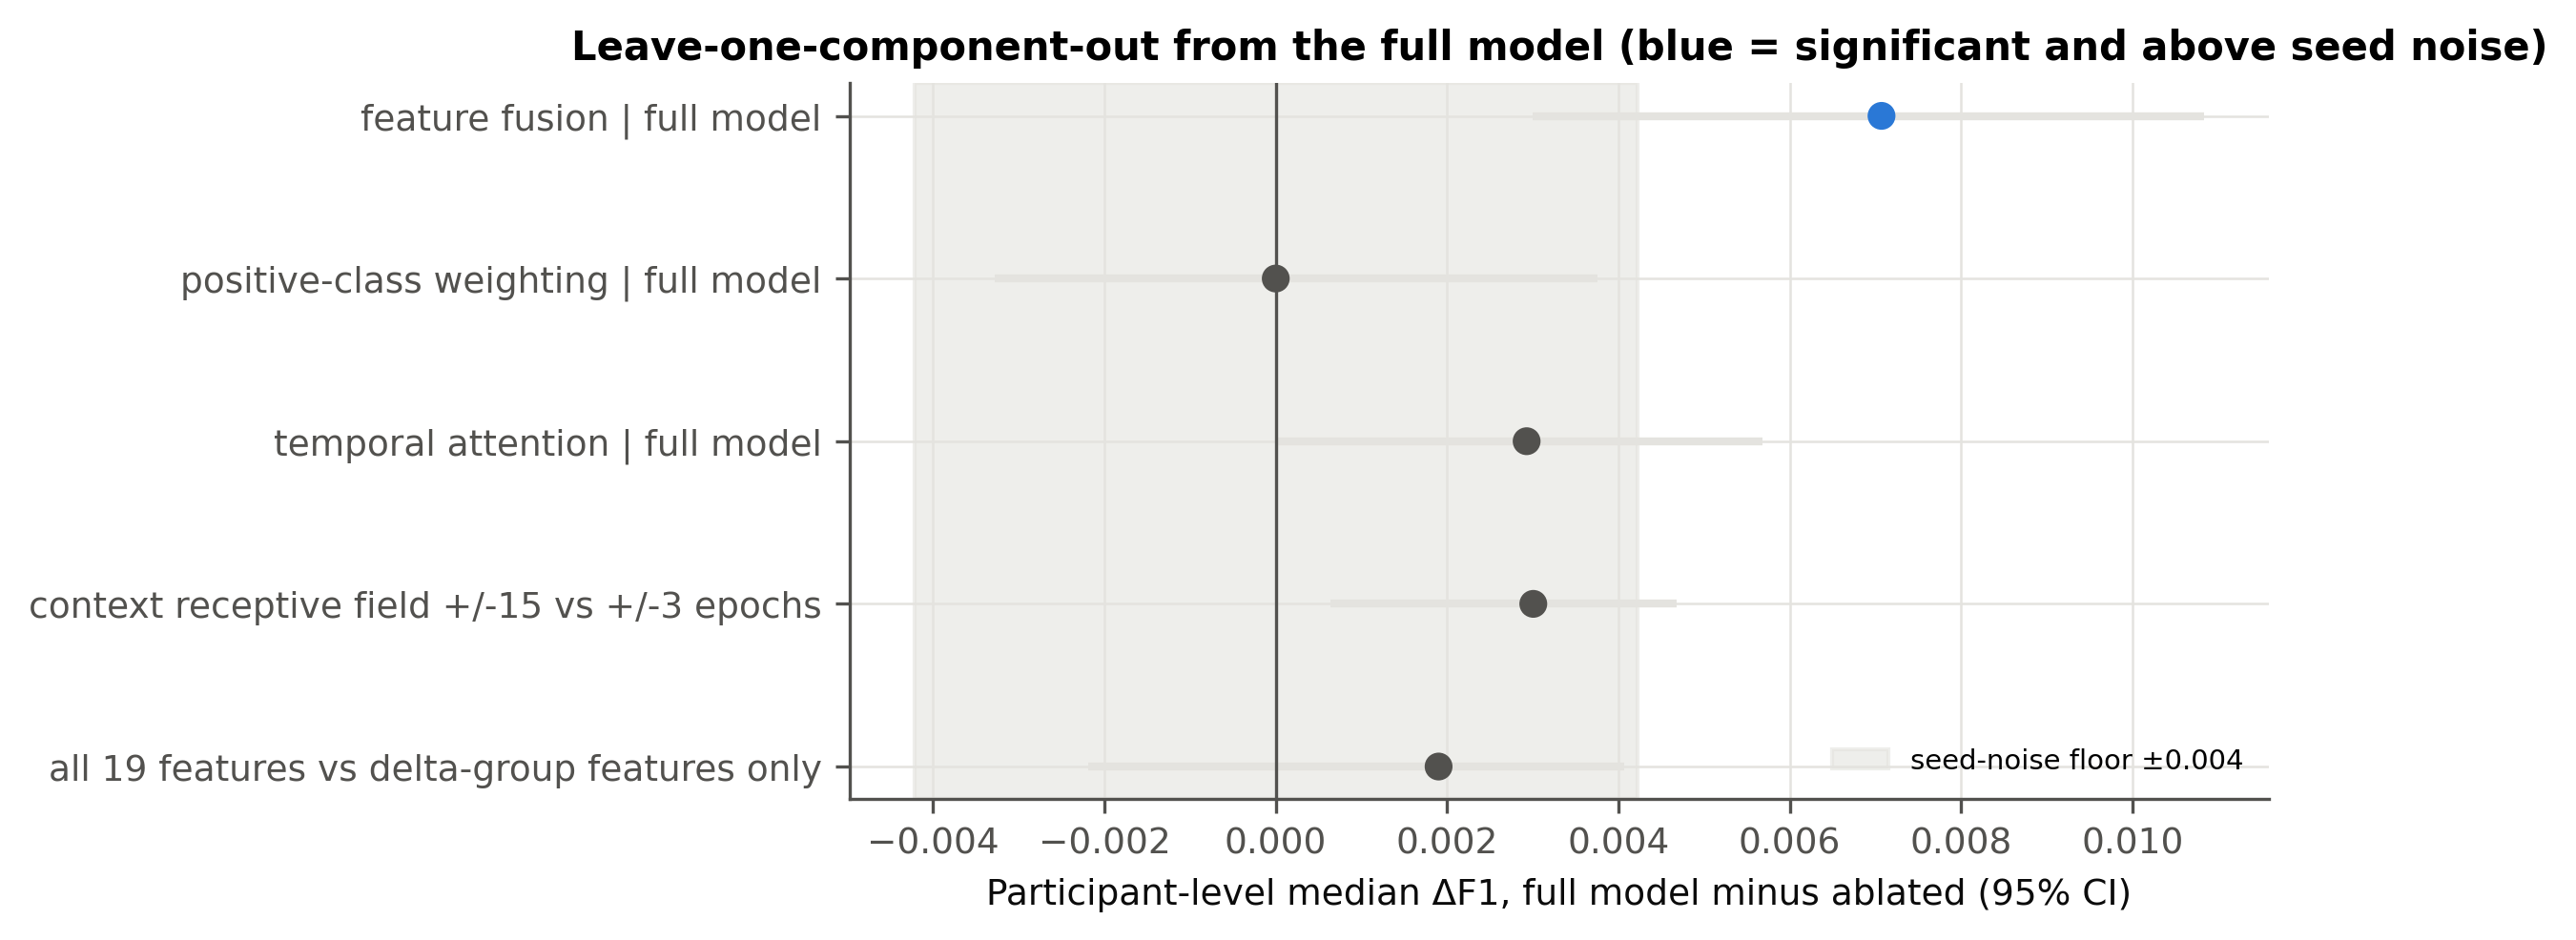
\includegraphics[width=0.86\columnwidth]{fig_rq4x_leave_one_out.png}
\caption{\textbf{[post hoc]} Post hoc leave-one-component-out from the full model. The shaded band is the largest seed-to-seed difference of the primary model.}
\end{figure}

\begin{table}[!t]
\caption{Intraclass correlation ICC(2,1) with McGraw--Wong 95\% confidence intervals for overnight-profile agreement (predicted vs expert hypnogram) and ISRUC-II test--retest.}
\centering\scriptsize
\begin{tabular}{@{}llccr@{}}
\toprule
Set & Quantity & ICC & 95\% CI & $n$ \\
\midrule
CV & N3 minutes & 0.806 & 0.76 to 0.85 & 251 \\
CV & Longest episode & 0.780 & 0.72 to 0.83 & 251 \\
CV & Episodes & 0.622 & 0.53 to 0.70 & 251 \\
CV & Median rating & 0.950 & 0.94 to 0.96 & 249 \\
CAP & N3 minutes & 0.730 & 0.63 to 0.81 & 105 \\
CAP & Longest episode & 0.765 & 0.67 to 0.83 & 105 \\
CAP & Episodes & 0.700 & 0.59 to 0.79 & 105 \\
CAP & Median rating & 0.888 & 0.83 to 0.93 & 105 \\
DOD-H & N3 minutes & 0.403 & -0.07 to 0.77 & 25 \\
DOD-H & Longest episode & 0.542 & -0.04 to 0.81 & 25 \\
DOD-H & Episodes & 0.381 & -0.10 to 0.71 & 25 \\
DOD-H & Median rating & 0.721 & -0.07 to 0.93 & 24 \\
DOD-O & N3 minutes & 0.222 & -0.08 to 0.55 & 55 \\
DOD-O & Longest episode & 0.294 & -0.10 to 0.61 & 55 \\
DOD-O & Episodes & 0.323 & -0.03 to 0.58 & 55 \\
DOD-O & Median rating & 0.745 & 0.27 to 0.89 & 53 \\
ISRUC-II night 1 & N3 minutes & 0.898 & 0.57 to 0.98 & 8 \\
ISRUC-II night 2 & N3 minutes & 0.740 & 0.20 to 0.94 & 8 \\
ISRUC-II night 1 & Median rating & 0.991 & 0.96 to 1.00 & 8 \\
ISRUC-II night 2 & Median rating & 0.989 & 0.94 to 1.00 & 7 \\
ISRUC-III & N3 minutes & 0.794 & 0.05 to 0.95 & 10 \\
ISRUC-III & Longest episode & 0.922 & 0.72 to 0.98 & 10 \\
ISRUC-III & Episodes & 0.478 & -0.07 to 0.83 & 10 \\
ISRUC-III & Median rating & 0.784 & -0.00 to 0.95 & 10 \\
Retest ISRUC-II & Rating & 0.763 & 0.23 to 0.95 & 8 \\
Retest ISRUC-II & Predicted N3 min & 0.658 & 0.01 to 0.92 & 8 \\
Retest ISRUC-II & Expert N3 min & -0.008 & -0.63 to 0.65 & 8 \\
Retest ISRUC-II & Delta intensity & 0.791 & 0.32 to 0.95 & 8 \\
Retest ISRUC-II & Morphology & 0.754 & 0.23 to 0.94 & 8 \\
Retest ISRUC-II & Spectral dominance & 0.339 & -0.26 to 0.80 & 8 \\
\bottomrule
\end{tabular}
\end{table}

\begin{figure}[!t]
\centering
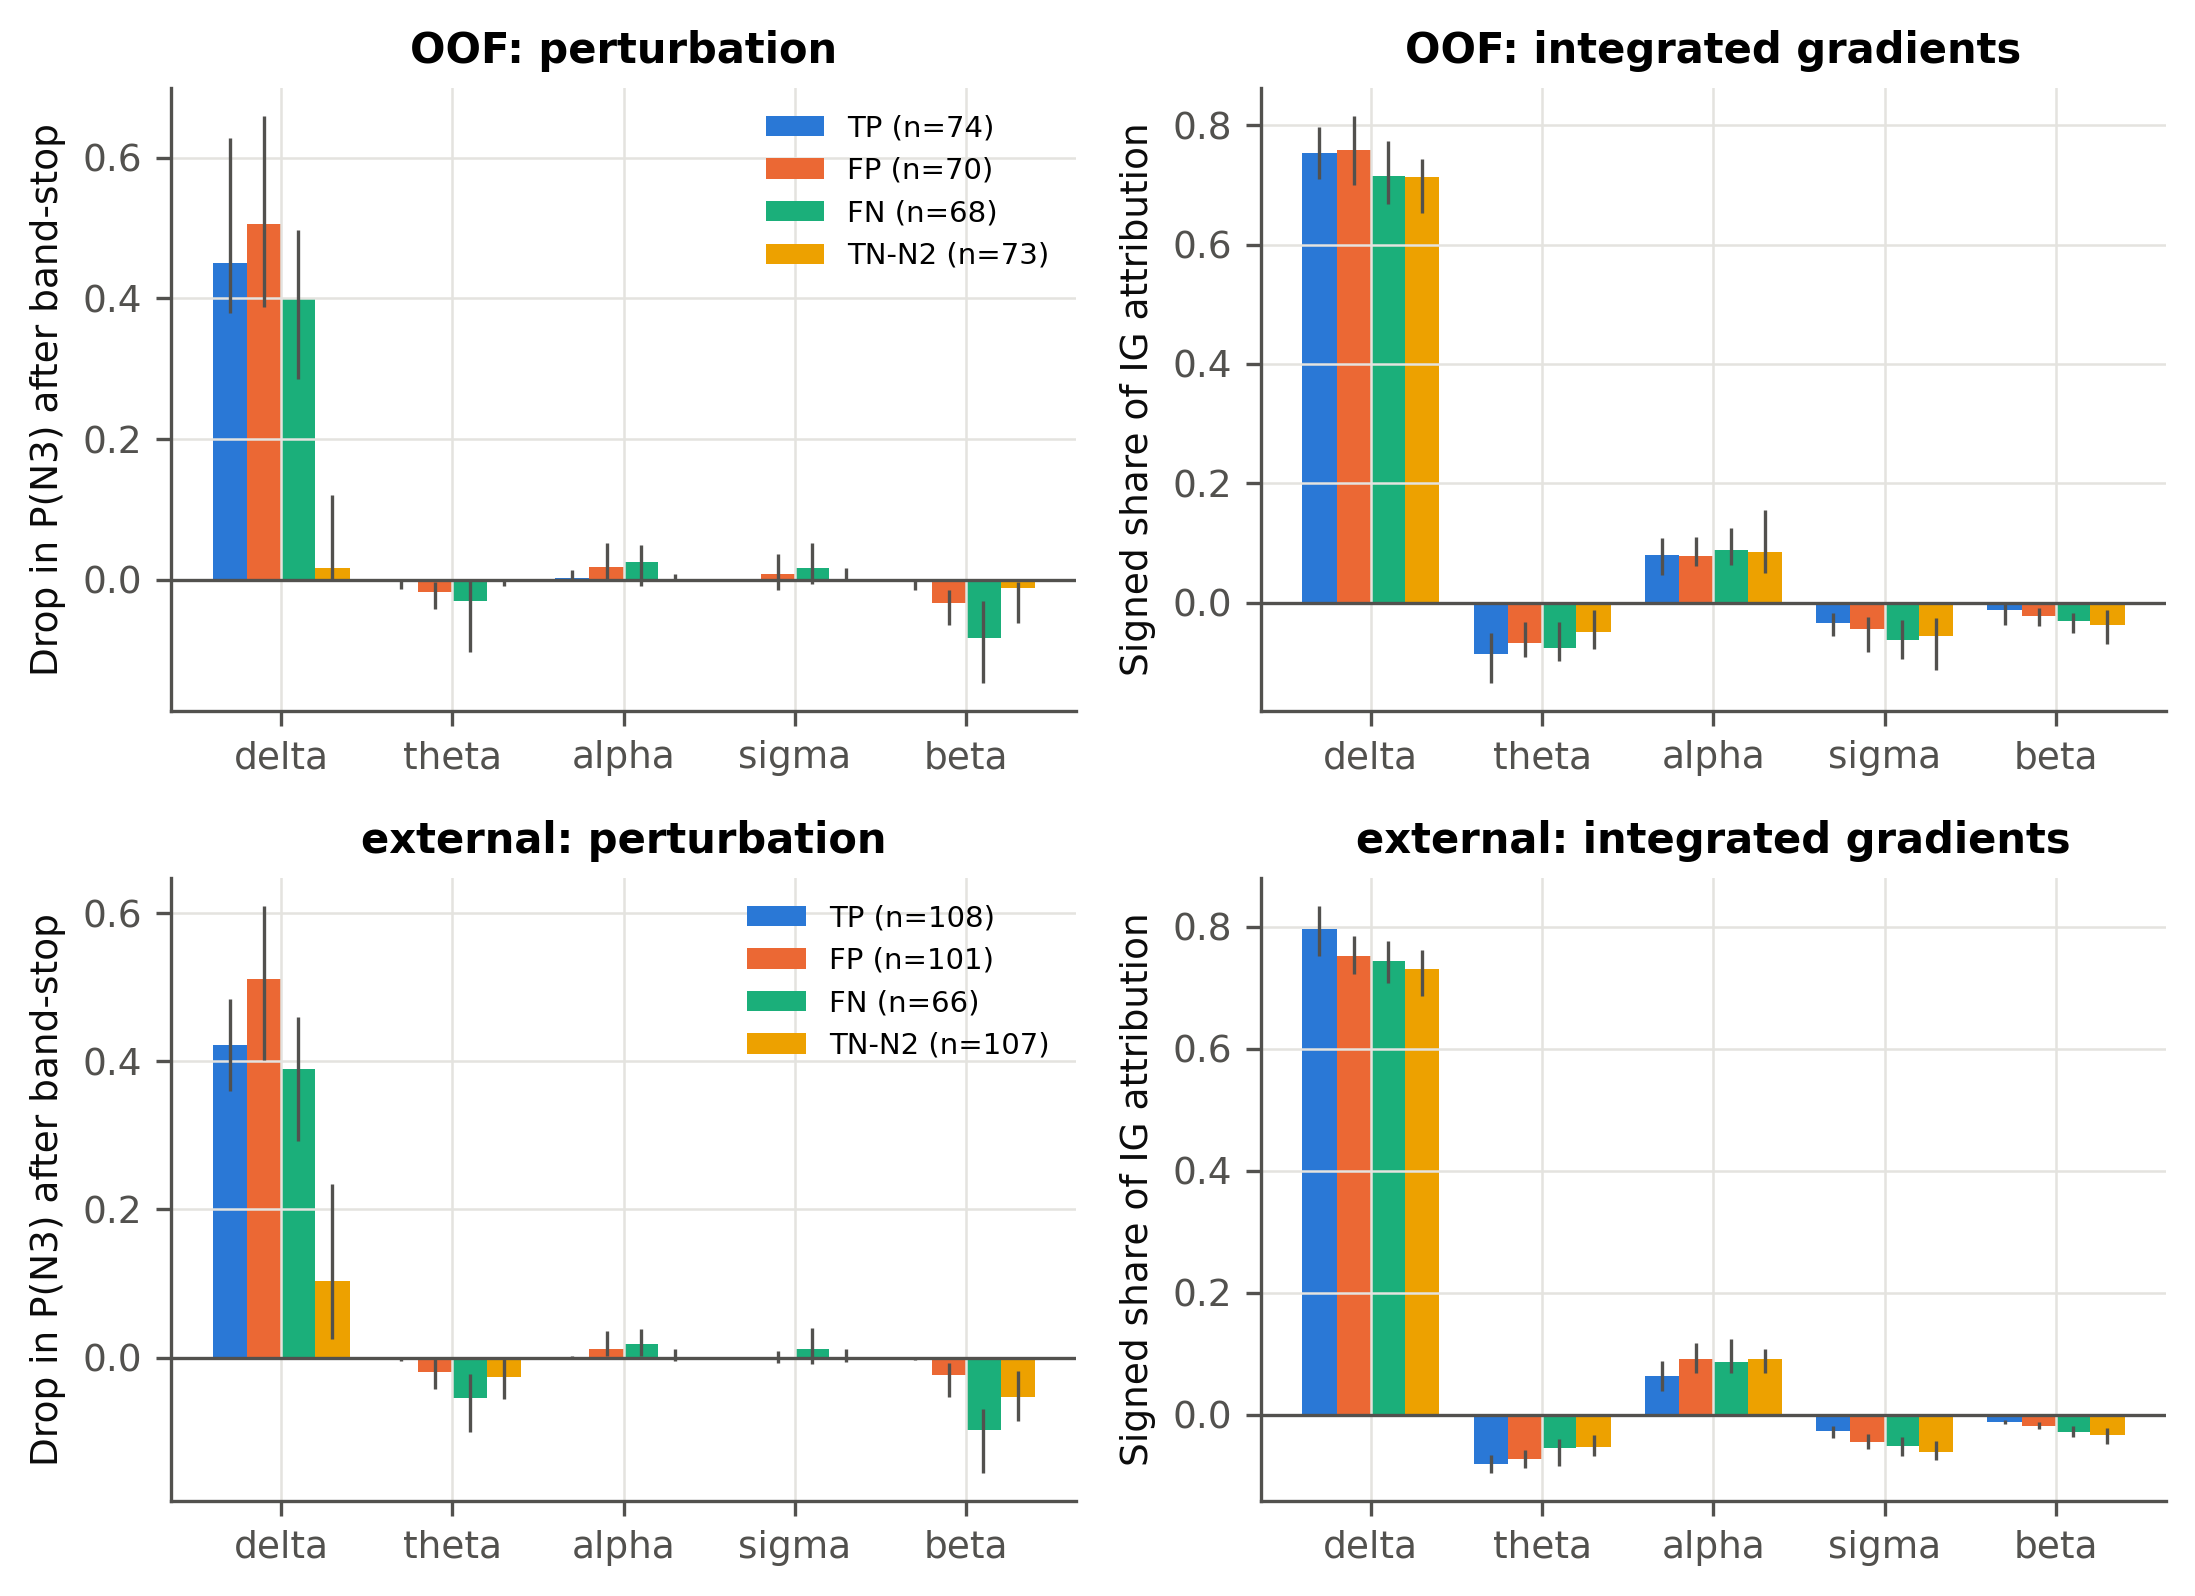
\includegraphics[width=0.86\columnwidth]{fig_rq5x_band_by_outcome.png}
\caption{\textbf{[post hoc]} Post hoc band importance by outcome (true and false positives, false negatives, true-negative N2 epochs) in cross-validation and external cohorts.}
\end{figure}

\begin{figure}[!t]
\centering
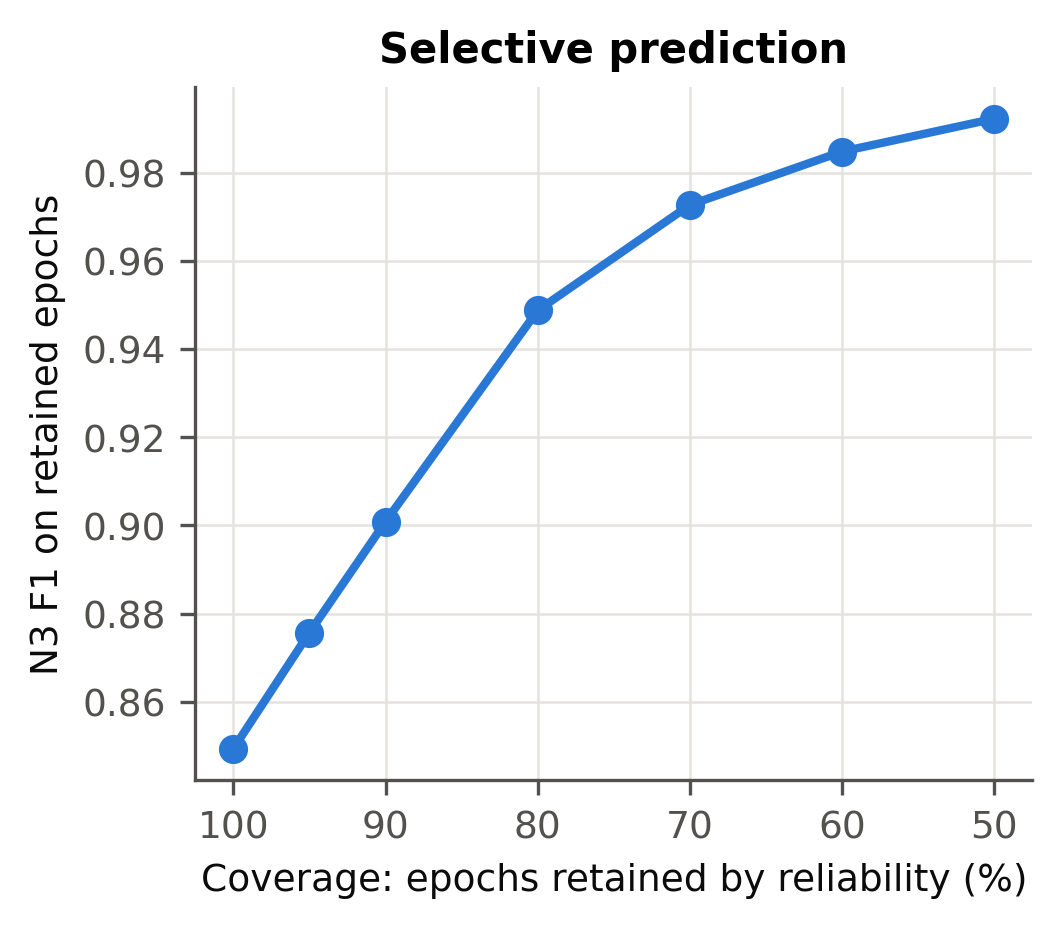
\includegraphics[width=0.7\columnwidth]{fig_rq6_risk_coverage.png}
\caption{N3 F1 score on the epochs retained when the least reliable epochs are withheld (cross-validation).}
\end{figure}

\begin{table}[!b]
\caption{Error-detection area under the ROC curve of each reliability input and of the cross-fitted combined score (cross-validation), and of the combined score in external cohorts.}
\centering\scriptsize
\begin{tabular}{@{}lc@{\hspace{12pt}}lc@{}}
\toprule
Input & Area & Set (combined) & Area \\
\midrule
Confidence & 0.872 & CAP & 0.853 \\
MC-dropout entropy & 0.879 & ISRUC-II & 0.872 \\
Mutual information & 0.800 & ISRUC-III & 0.941 \\
Mahalanobis distance & 0.855 & DOD-H & 0.751 \\
QC score & 0.480 & DOD-O & 0.689 \\
QC high-frequency ratio & 0.297 & ISRUC-I disagreement & 0.883 \\
QC clipping & 0.479 & External disagreement & 0.628 \\
Any QC flag & 0.447 & & \\
Combined & 0.879 & & \\
\bottomrule
\end{tabular}
\end{table}

\begin{figure}[!t]
\centering
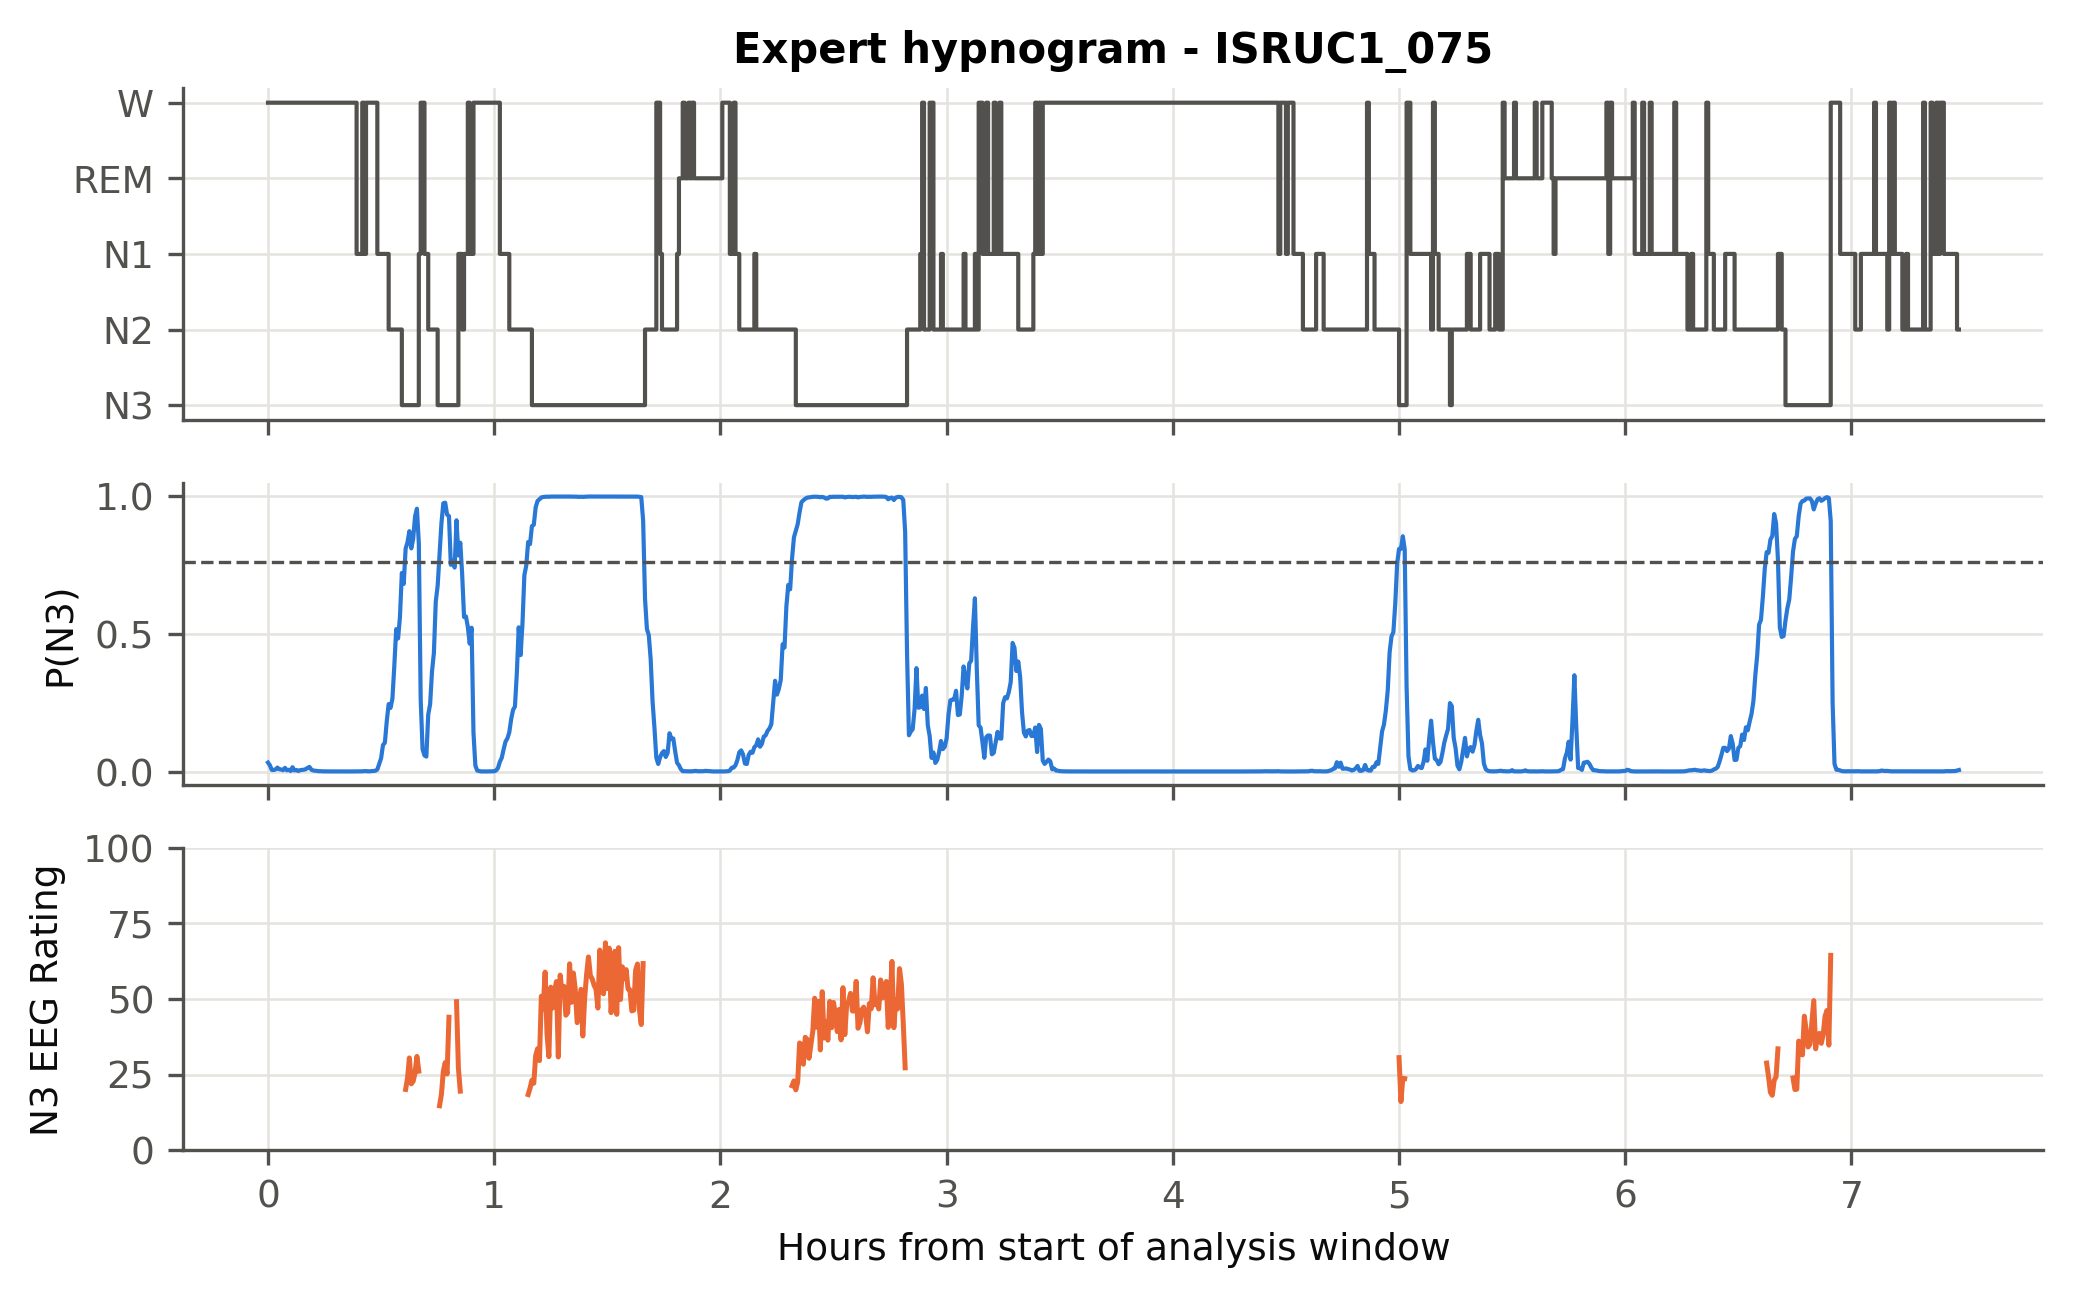
\includegraphics[width=0.86\columnwidth]{fig_example_overnight_profile.png}
\caption{One ISRUC-I night: expert hypnogram, N3 probability with the decision threshold (dashed), and the N3 EEG rating of detected epochs.}
\end{figure}

\begin{table}[!t]
\caption{\textbf{[Robustness, post hoc]} Post hoc sensitivity analyses: number of settings that test a conclusion and number in which it holds.}
\centering\scriptsize
\begin{tabular}{@{}llrr@{}}
\toprule
Question & Analysis & Tested & Holds \\
\midrule
Detection & decision threshold & 8 & 7 \\
Detection & reference standard & 25 & 20 \\
Detection & quality control & 8 & 7 \\
Detection & participant-level summary & 8 & 7 \\
Factor validity & early $>$ late-night decline & 65 & 48 \\
Grade & stage 4 vs 3 area & 1 & 1 \\
Stability & weighting, factor removal & 8 & 7 \\
Components & leave-one-component-out & 5 & 1 \\
Explanations & baselines, steps, outcomes, bootstrap & 11 & 11 \\
Reliability & error detection per cohort & 9 & 8 \\
Profile & N3 minutes ICC & 16 & 10 \\
Profile & episode definition & 16 & 2 \\
\bottomrule
\end{tabular}
\end{table}

\end{document}
